\section{WebProtelis}

  % TODO: dovrei reinserire il diagramma grosso???
  % \begin{frame}{\insertsectionhead}
  %   \begin{figure}
  %     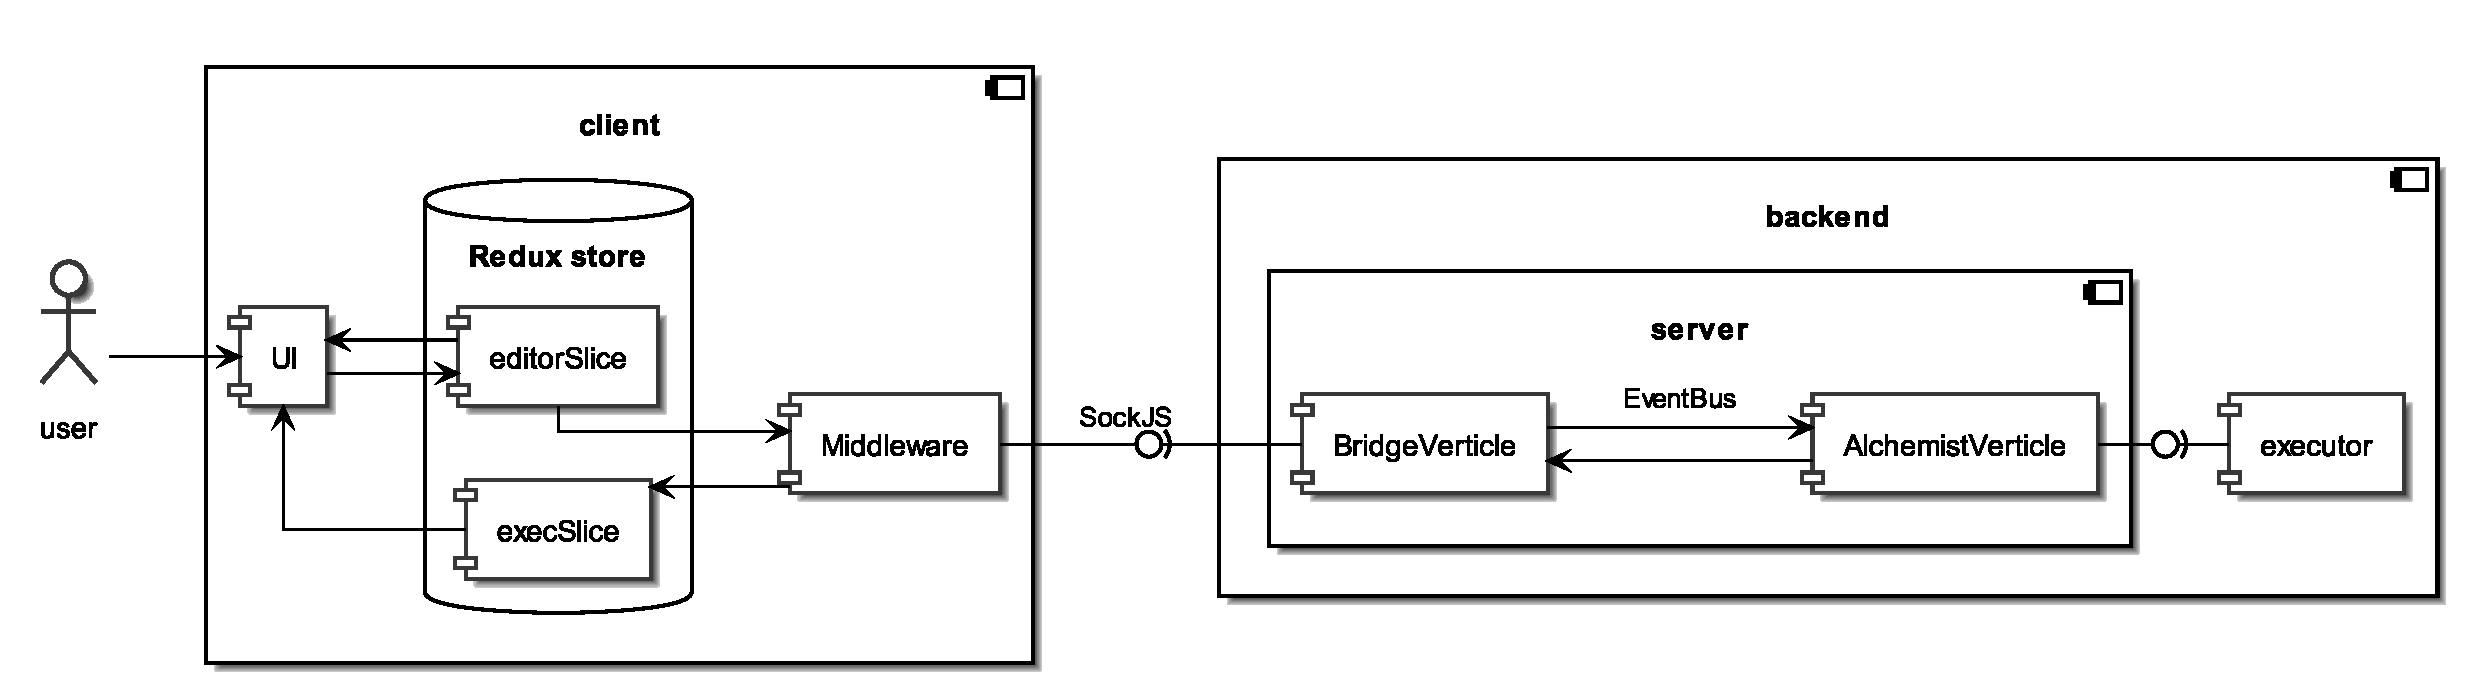
\includegraphics[width=\textwidth]{res/uml/architecture-design-detail.eps}
  %   \end{figure}
  % \end{frame}

  \subsection{Progettazione del server}

    \begin{frame}{\insertsectionhead}{\insertsubsectionhead}

      % \begin{columns}
        % \begin{column}{.55\textwidth}
          \begin{block}{Servizi offerti}
            Il backend mette a disposizione due funzionalità principali:
            \begin{itemize}
              \item API per la comunicazione remota
              \item esecutore del codice Protelis
            \end{itemize}
          \end{block}
        % \end{column}
        % \begin{column}{.4\textwidth}
          \begin{figure}
            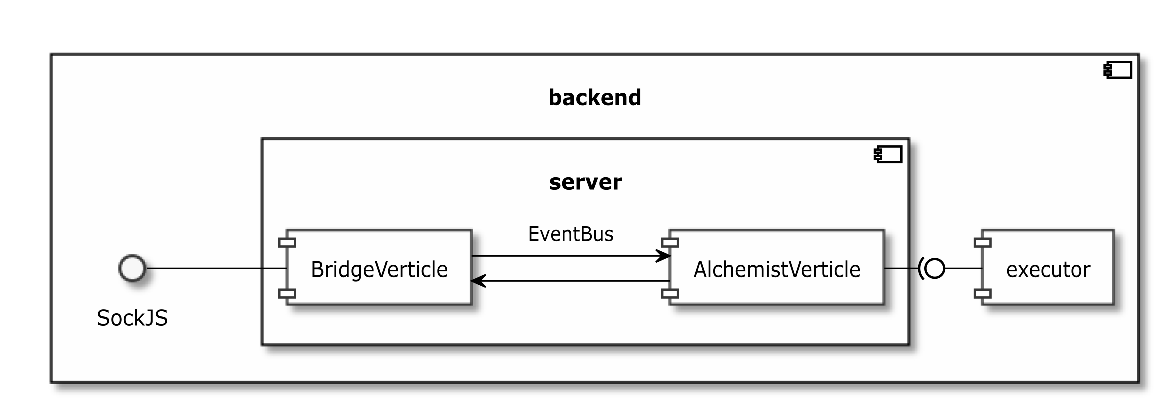
\includegraphics[width=.67\textwidth]{res/uml/architecture-design-server.eps}
          \end{figure}
        % \end{column}
      % \end{columns}
    \end{frame}

    \begin{frame}{\insertsectionhead}
      \framesubtitle{\insertsubsectionhead}

      \begin{columns}
        \begin{column}{.8\textwidth}
          \begin{block}{Vert.x}
            \strong{Vert.x} è un framework applicativo reattivo e event-driven per JVM.

            Caratteristiche principali:
            \begin{itemize}
              \item<2-> reattivo e basato su pattern Multi-Reactor
              \item<3-> supporto a costrutti \emph{actor-like} detti \strong{Verticle}
              \item<4-> supporto a comunicazione tramite EventBus
            \end{itemize}

            % Del modello architetturale messo a disposizione dal framework, è stato considerato interessante il concetto di \emph{Verticle}:
            % esso è un'astrazione, simile al pattern ad attori ma non considerato pienamente aderente al modello teorico dalla stessa documentazione ufficiale,
            % che incapsula un event-loop insieme al suo stato e interagisce tramite gli eventi provenienti da un EventBus.
          \end{block}
        \end{column}
        \begin{column}{.15\textwidth}
          \begin{figure}
            
\includegraphics[width=\textwidth]{res/uml/vertx-logo-big.png}
          \end{figure}
        \end{column}
      \end{columns}

      \begin{columns}
        \begin{column}{.99\textwidth}
          \begin{block}<5->{Verticle modellati}
            \begin{itemize}
              \item \texttt{BridgeVerticle} gestisce le API attraverso \emph{SockJS} e \emph{EventBus}
              \item \texttt{AlchemistVerticle} costruisce e monitora simulazioni Alchemist per eseguire il codice Protelis
            \end{itemize}
          \end{block}
        \end{column}
      \end{columns}
    \end{frame}

    \subsection{Progettazione del client}

    % \begin{frame}{\insertsectionhead}{\insertsubsectionhead}
    %   \begin{block}{Struttura}
    %     \begin{itemize}
    %       \item<1-> Il client dovrebbe essere una Single-Page Application composta da un editor e da un canvas
    %       \item<2-> Simile a CodeSandbox\onslide<3->{, TypeScript Playground }\onslide<4->{o Overleaf}
    %     \end{itemize}
    %   \end{block}

    %   \begin{figure}
    %     \centering
    %     \only<2>{%
    %       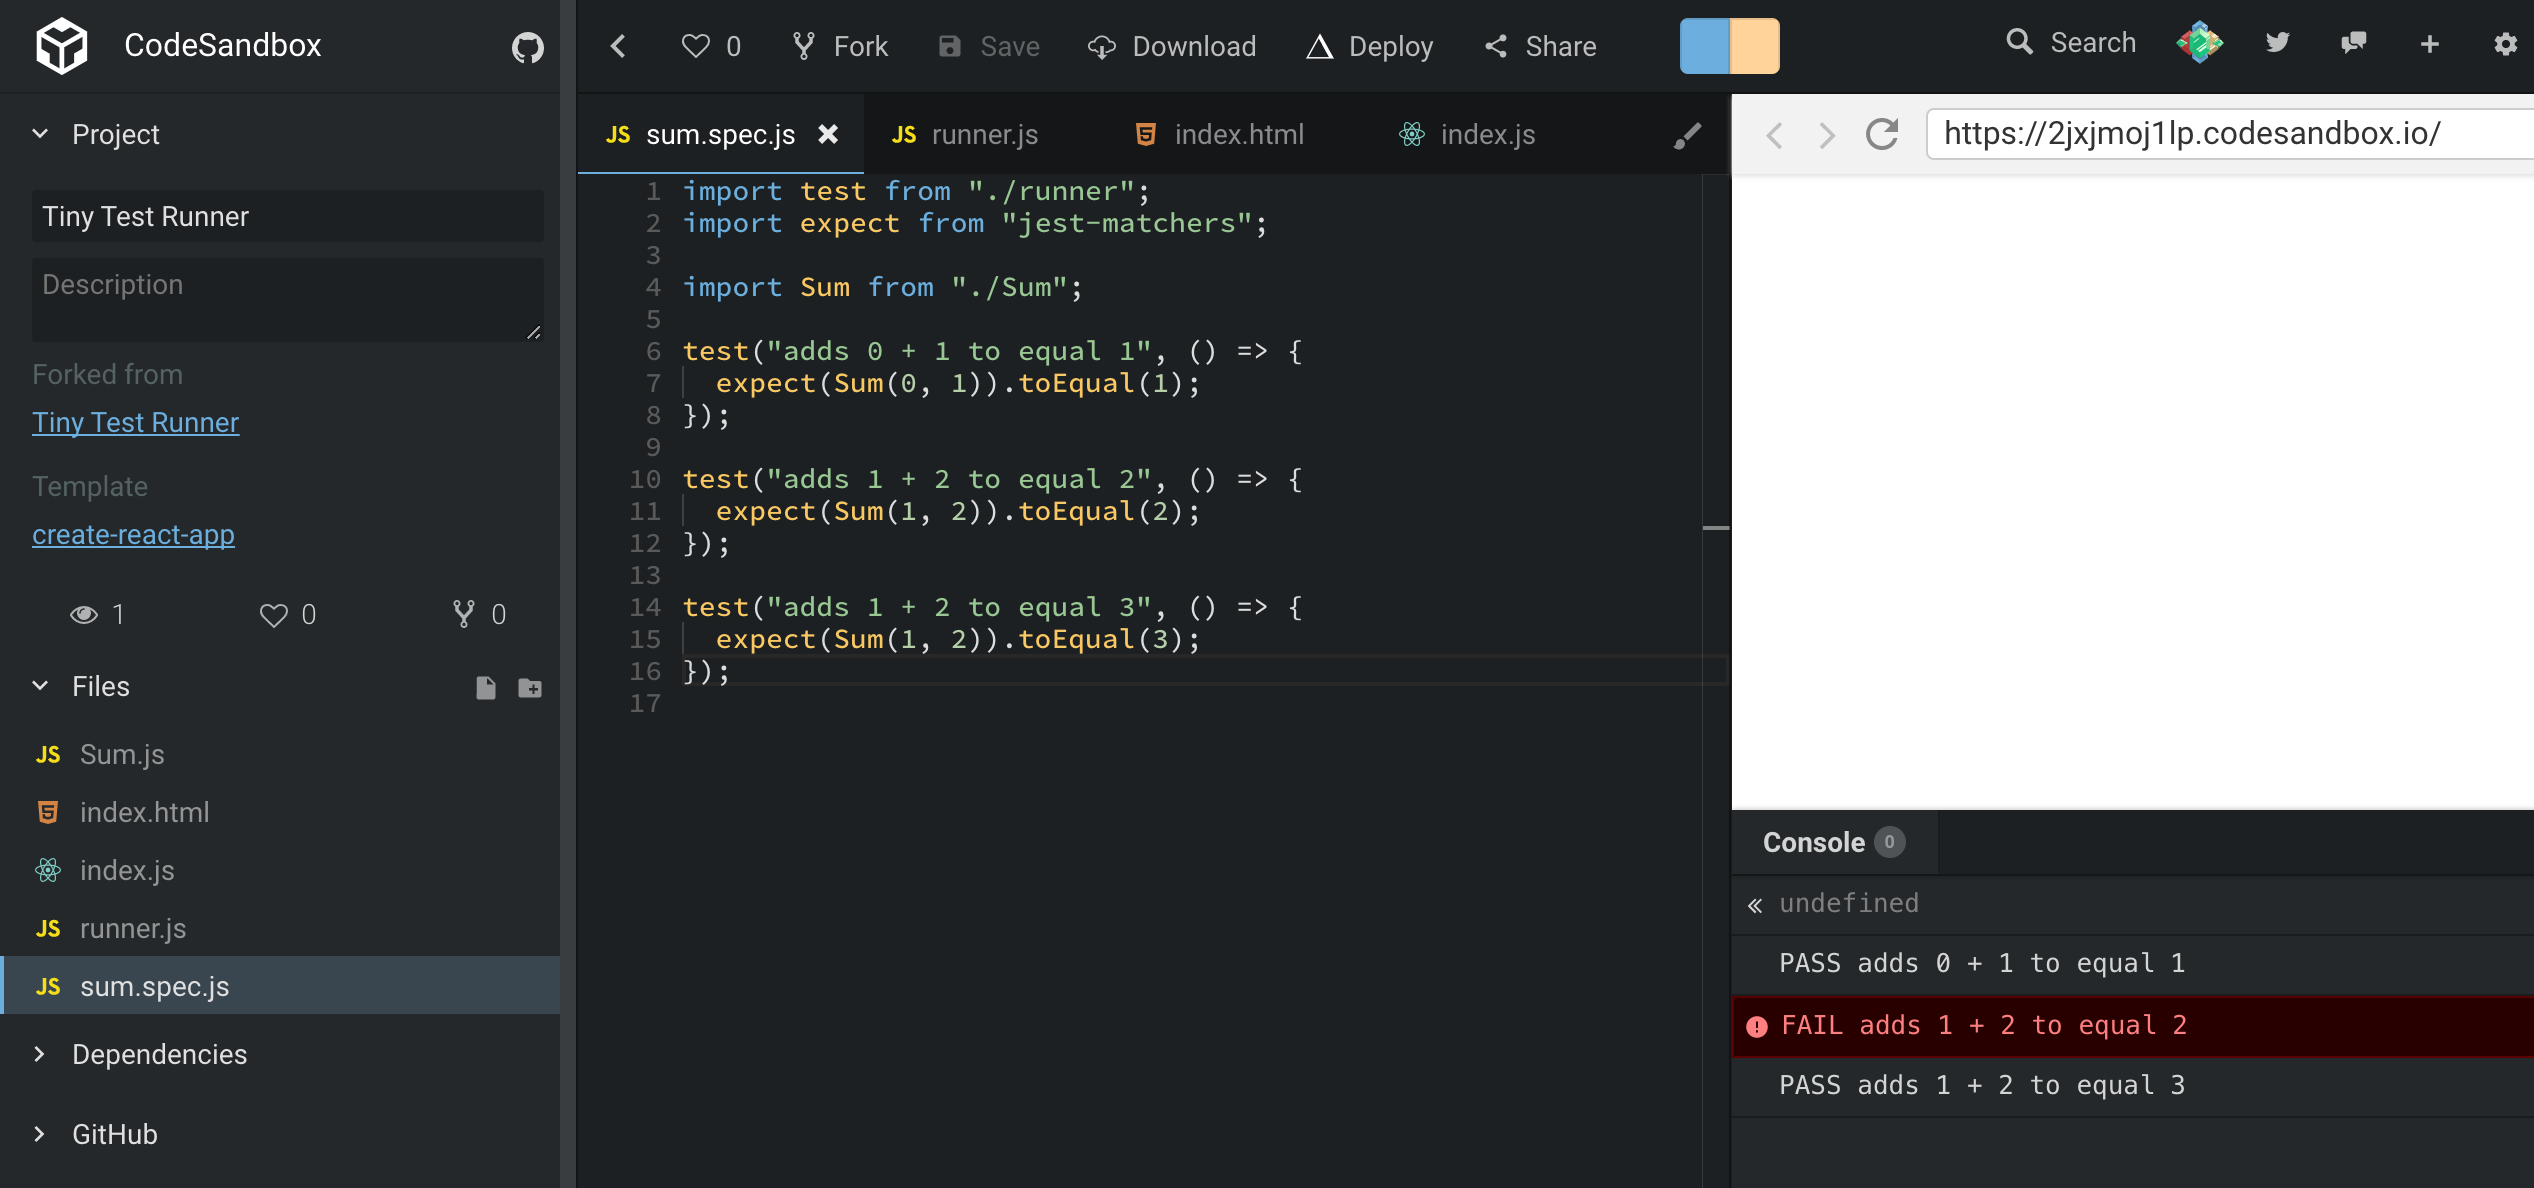
\includegraphics[width=.5\textwidth]{res/fig/codesandbox.png}%
    %     }%
    %     \only<3>{%
    %       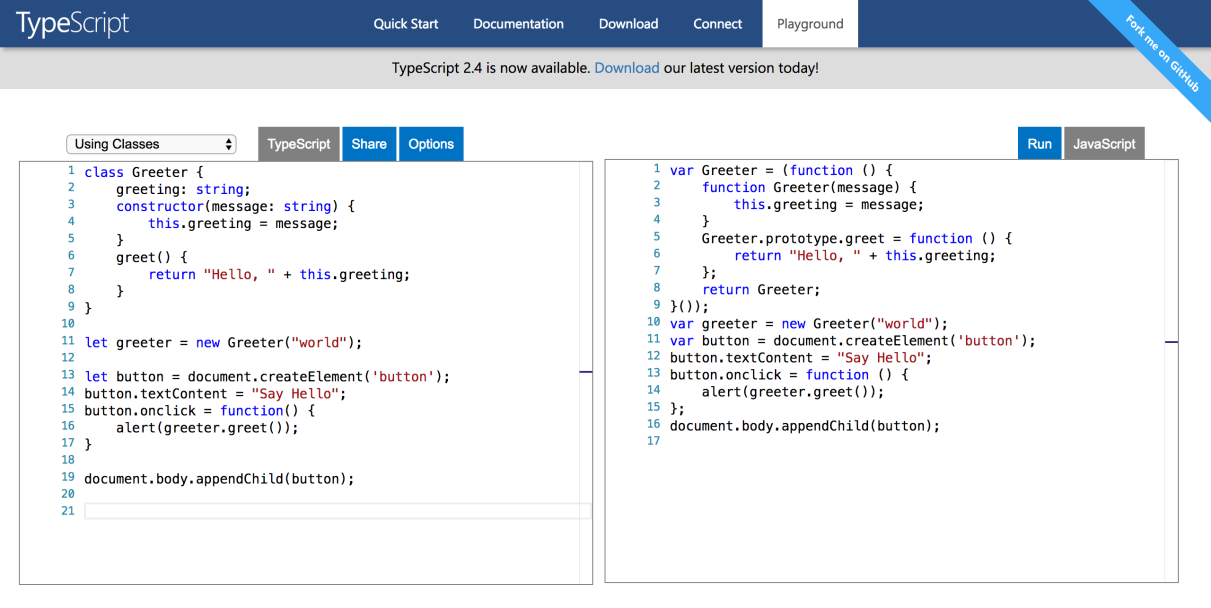
\includegraphics[width=.5\textwidth]{res/fig/typescript-playground.png}%
    %     }%
    %     \only<4>{%
    %       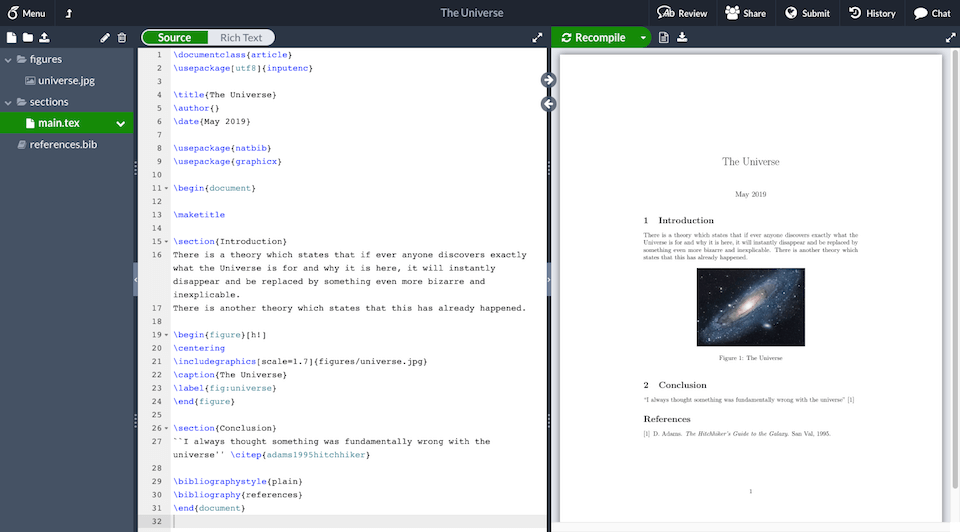
\includegraphics[width=.5\textwidth]{../res/fig/overleaf.png}%
    %     }%
    %   \end{figure}
    % \end{frame}

    % \begin{frame}{\insertsectionhead}{\insertsubsectionhead{}: Mockup}
    %   \centering
    %   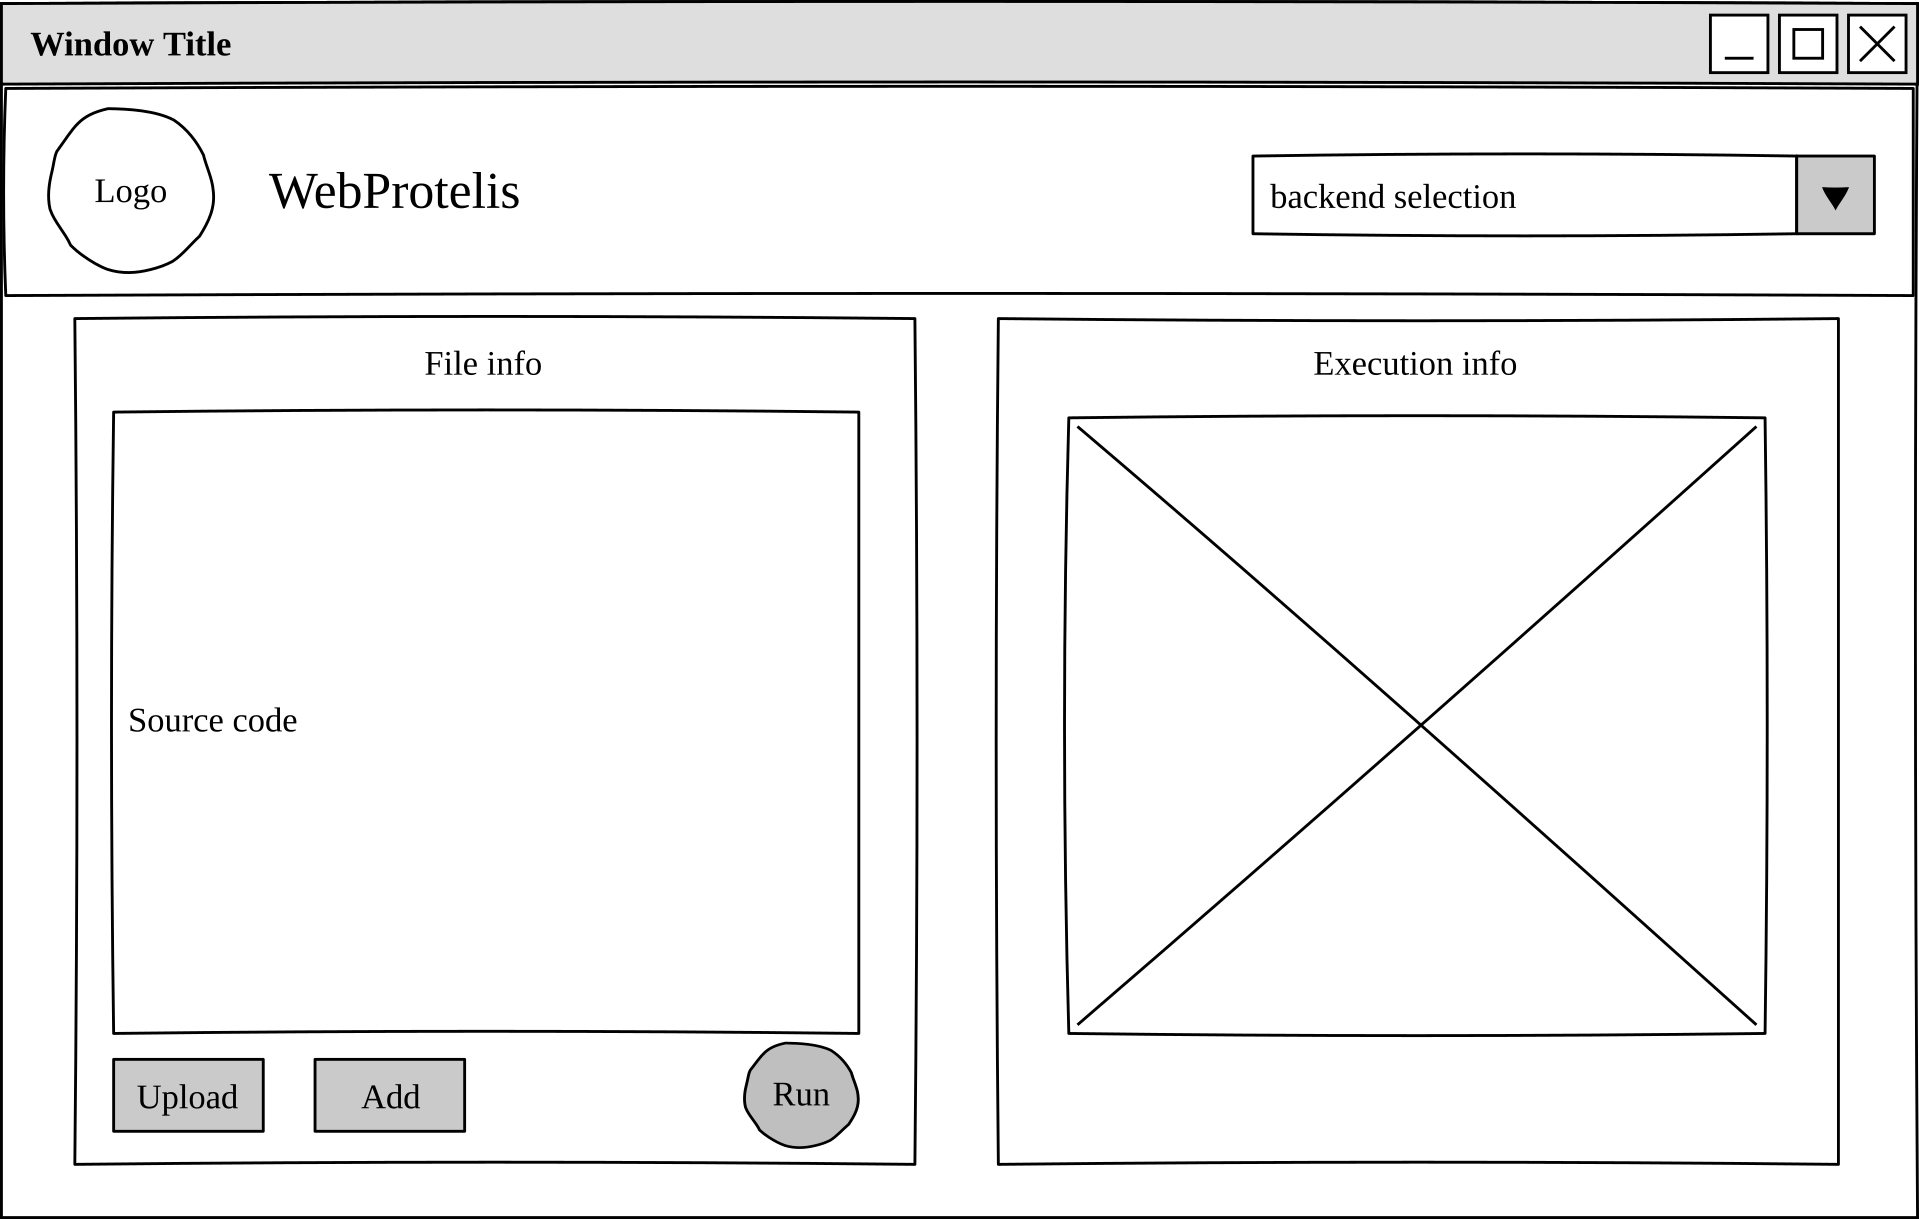
\includegraphics[width=.9\textwidth]{res/fig/gui-actual.png}
    % \end{frame}

    \begin{frame}{\insertsectionhead}{\insertsubsectionhead}
      \begin{columns}
        \begin{column}{.8\textwidth}
          \begin{block}{Framework}
            \begin{itemize}
              \item
                Per l'implementazione è stato scelto \strong{React}
                \begin{itemize}
                  \item React è una libreria per la costruzione di pagine web reattive e data-driven
                  \item Suddivide la pagina in componenti, gestiti tramite struttura ad albero
                  \item Tramite un sistema di dipendenze, determina in modo reattivo cosa deve essere renderizzato nuovamente
                \end{itemize}
              \item
                Fondamentale pianificare la gestione dello \strong{stato}
            \end{itemize}
          \end{block}
        \end{column}
        \begin{column}{.15\textwidth}
          \begin{figure}
            
\includegraphics[width=\textwidth]{res/uml/react-logo.png}
          \end{figure}
        \end{column}
      \end{columns}
    \end{frame}

    \begin{frame}{\insertsectionhead}{\insertsubsectionhead}
      \begin{columns}
        \begin{column}{.5\textwidth}
          \begin{block}{Gestione dello stato}
            \begin{itemize}
              \item<1->
                Facebook propone un pattern architetturale alternativo a MVC:
                \strong{Flux}
              \item<2->
                \strong{Redux} è una delle più popolari varianti
            \end{itemize}
          \end{block}
          \begin{block}<3->{Componenti e stato}
            Sono state individuate due \emph{slice} dello stato, relativamente ai due elementi di layout principali:
            \begin{itemize}
              \item<3-> \texttt{editorSlice}
              \item<4-> \texttt{execSlice}
            \end{itemize}
          \end{block}
        \end{column}
        \begin{column}{.45\textwidth}
          \begin{figure}
            \includegraphics<2>[width=.9\textwidth]{../res/fig/redux-diagram.png}
            \includegraphics<3->[width=.9\textwidth]{res/uml/architecture-design-client.eps}
          \end{figure}
        \end{column}
      \end{columns}
    \end{frame}

    % \begin{frame}{\insertsectionhead}{\insertsubsectionhead}

    %   \begin{columns}
    %     \begin{column}{.5\textwidth}
    %       \begin{block}{Componenti e stato}
    %         Sono state individuate due \emph{slice} dello stato, relativamente ai due elementi di layout principali:
    %         \begin{itemize}
    %           \item<2-> \texttt{editorSlice}
    %           \item<3-> \texttt{execSlice}
    %         \end{itemize}
    %       \end{block}
    %     \end{column}
    %     \begin{column}{.45\textwidth}
    %       \begin{figure}
    %         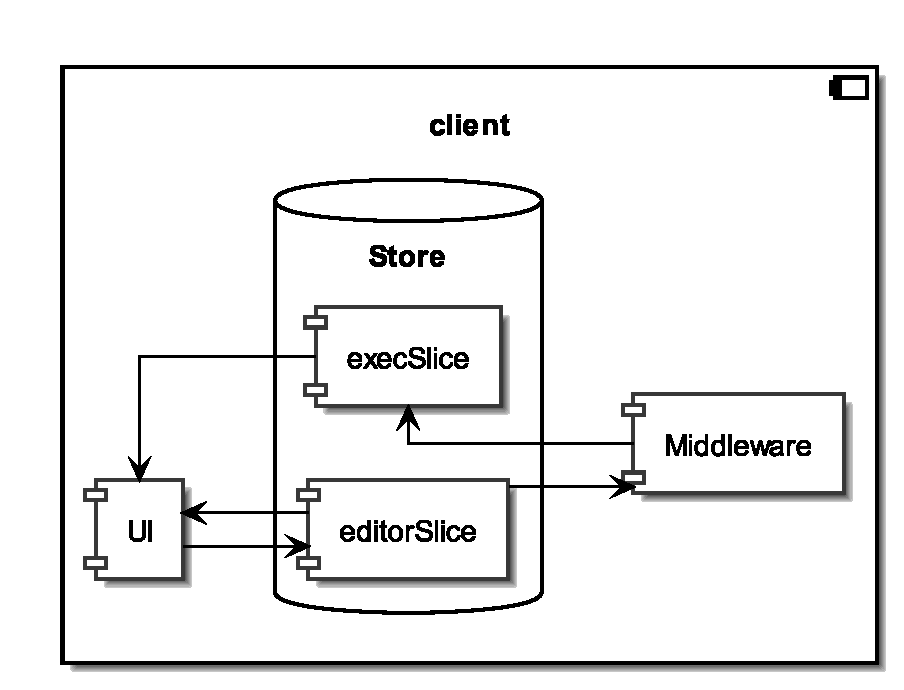
\includegraphics[width=.9\textwidth]{res/uml/architecture-design-client.eps}
    %       \end{figure}
    %     \end{column}
    %   \end{columns}

    %   \begin{figure}
    %     \centering
    %     \only<2>{%
    %       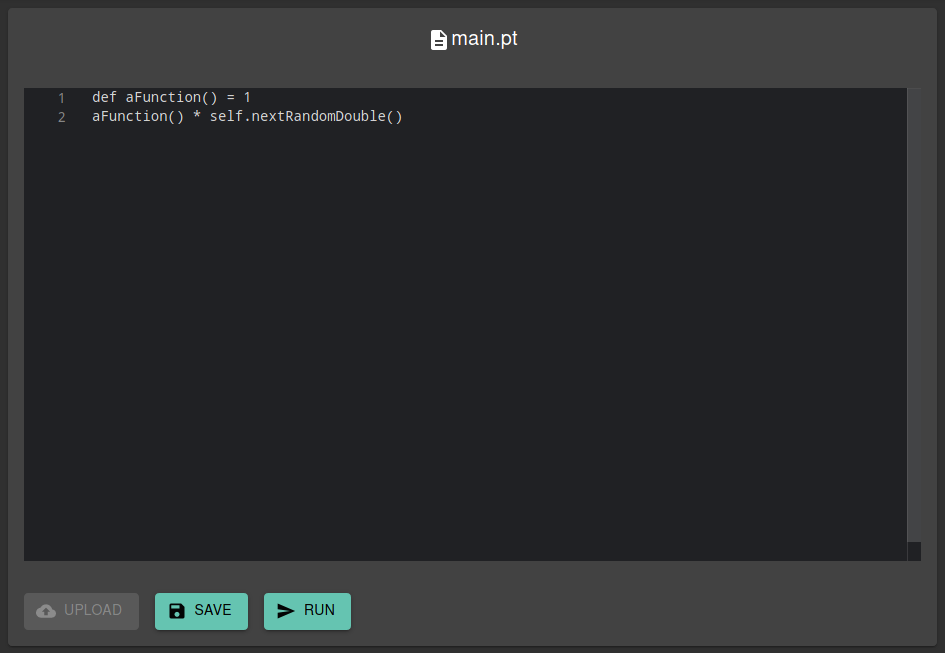
\includegraphics[width=.65\textwidth]{../res/screenshot/Screenshot_2020-03-02 Protelis on the Web(2).png}%
    %     }%
    %     \only<3>{%
    %       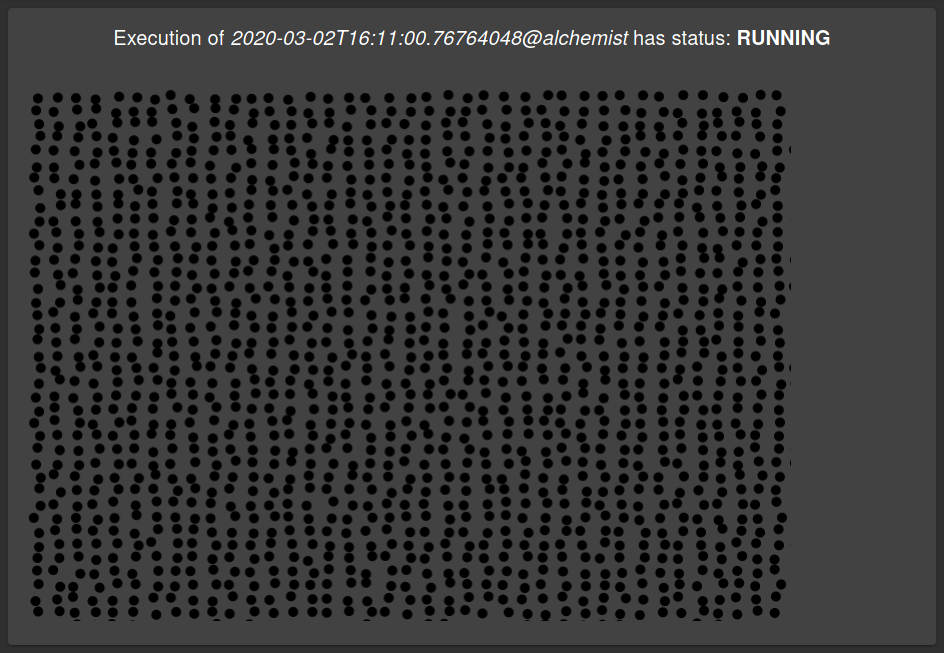
\includegraphics[width=.65\textwidth]{../res/screenshot/Screenshot_2020-03-02 Protelis on the Web(7).png}%
    %     }%
    %   \end{figure}
    % \end{frame}

  \subsection{Valutazione dei risultati}

    \begin{frame}{\insertsectionhead}{\insertsubsectionhead{}: Demo}
      \centering
      \includemedia[%
        width=.9\textwidth,%
        height=.35\textwidth,%
        keepaspectratio,%
        activate=onclick,%
        deactivate=pageclose,%
        passcontext,%
        transparent,%
        addresource=res/demo.mp4,%
        flashvars={source=res/demo.mp4}%
      ]{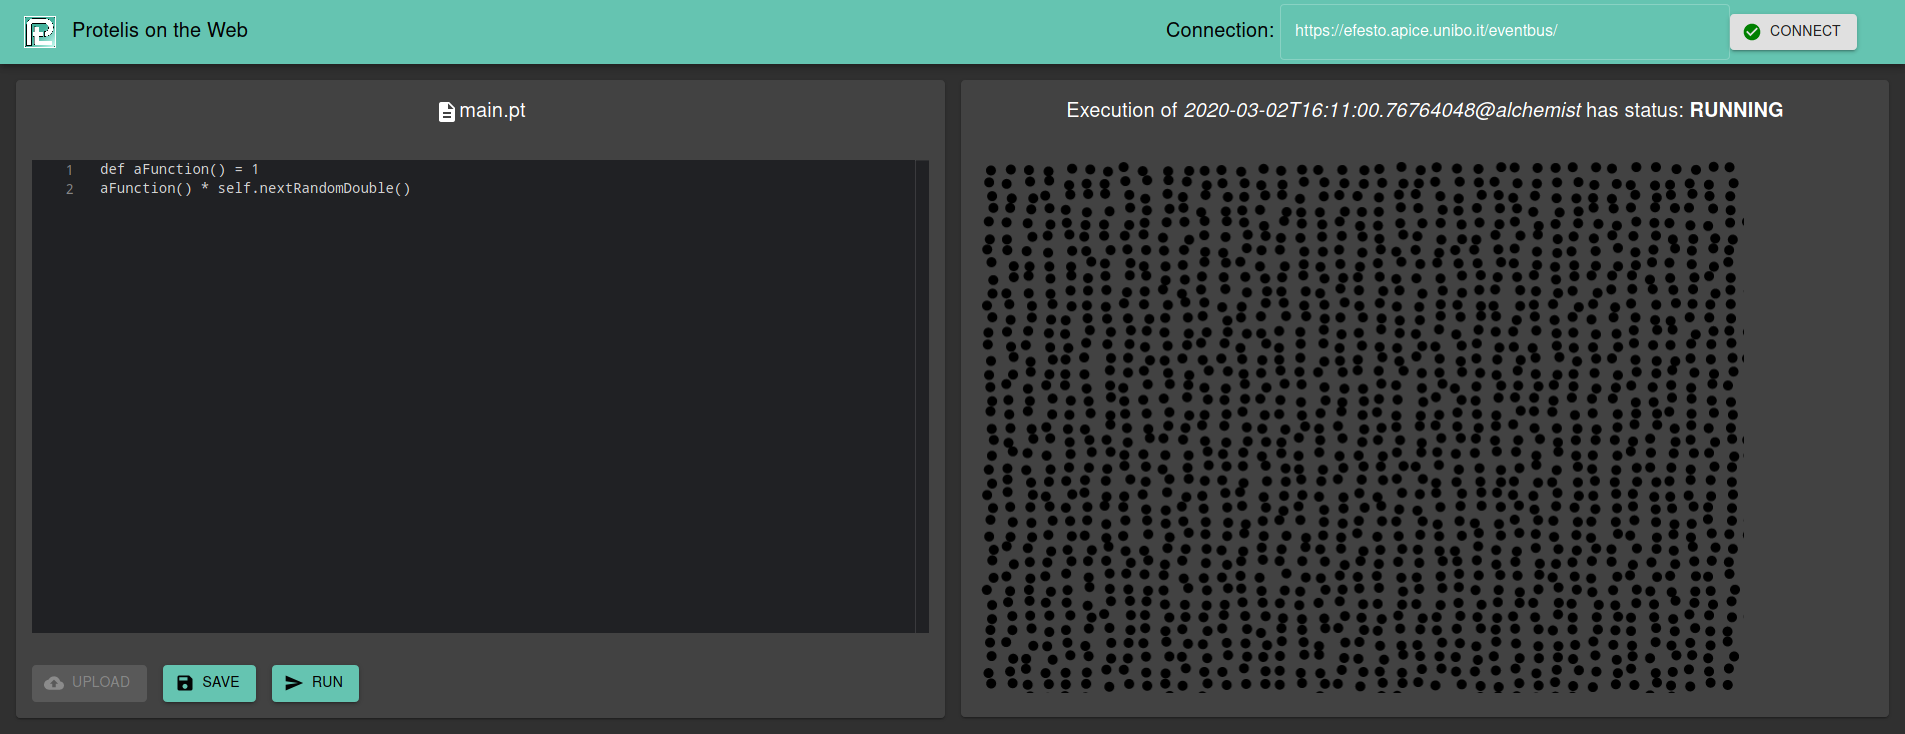
\includegraphics[width=.9\textwidth]{../res/screenshot/Screenshot_2020-03-02 Protelis on the Web(6).png}}{VPlayer.swf}
    \end{frame}

    \begin{frame}{\insertsectionhead}{\insertsubsectionhead{}: Google Lighthouse}
      \centering
      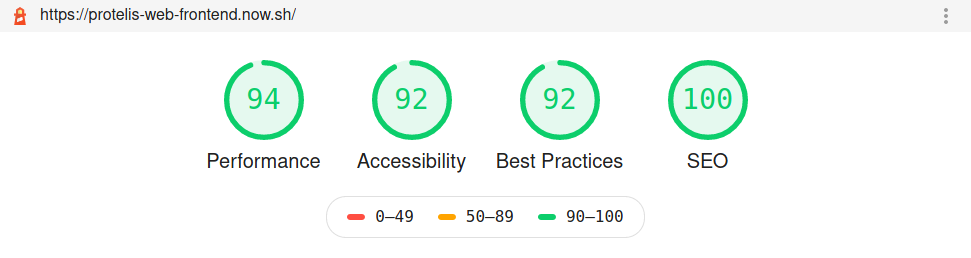
\includegraphics[width=\textwidth]{../res/tests/Screenshot_2020-03-04 Lighthouse Report Viewer.png}
    \end{frame}
